\documentclass[parskip=full,11pt]{scrartcl}
\usepackage[utf8]{inputenc}
\usepackage[T1]{fontenc}
\usepackage[german]{babel}
\usepackage[useregional]{datetime2}
\usepackage[pdfborderstyle={/S/U/W 0}]{hyperref}
\usepackage[nameinlink]{cleveref}
\usepackage[section]{placeins}
\usepackage{xcolor}
\usepackage{graphicx}
\usepackage{csquotes}
\usepackage{amsmath} % for $\text{}$
\usepackage{pflichtenheft}

\newcommand\urlpart[2]{$\underbrace{\text{\texttt{#1}}}{\text{#2}}$}

\crefname{figure}{Abb}{Abb}

\hypersetup{
	pdftitle={Pflichtenheft},
	bookmarks=true,
}

% section numbers in margins:
\renewcommand\sectionlinesformat[4]{\makebox[0pt][r]{#3}#4}

% header & footer
\usepackage{scrlayer-scrpage}
\lofoot{\today}
\refoot{\today}
\pagestyle{scrheadings}

\newcommand\producttitle{GO-App}

\title{Pflichtenheft: \producttitle}
\author{Lukas Dippon
        \and Jens Kienle
        \and Matthias Noll
        \and Fabian Röpke
        \and Tim Schmidt
        \and Simon Vögele}

\begin{document}
\maketitle

\section{Einleitung}
Studenten und Mitarbeiter des KIT treffen sich gerne zum gemeinsamen Essen oder Lernen.
Dazu ist an einem bestimmten Tag immer notwendig zu wissen, ob bereits ein Treffen vereinbart wurde.
Am Treffpunkt angekommen, möchte man wissen, an welchem Ort sich die Gruppe befindet, um nicht lange suchen zu müssen.
Unsere App soll es angemeldeten Benutzern ermöglichen, sich in Gruppen zu organisieren.
In den Gruppen kann der Zeit- und Treffpunkt bestimmt werden.
Nach der Festlegung des Treffens soll die App die GPS-Standorte der Mitglieder temporär und anonym anzeigen, um das Treffen zu vereinfachen.

\pagebreak
%%%%%%%%%%%%%%
\section{Kriterien}
% Diese Section sollte kurz und knapp "für Manager" sein
% und auf eine Seite passen.

\subsection{Muss}
\criterium{Gruppen}{crt:groups}{10}
Mehrere Nutzer können sich in Gruppen zusammenschließen.
Ein Nutzer kann in beliebig vielen Gruppen Mitglied sein.

\criterium{Eigene Position auf Umgebungskarten}{crt:location}{20}
Der Nutzer ist in der Lage, seine aktuelle Position auf einer Karte der nahen
Umgebung einzusehen.

\criterium{Festlegbare Treffpunkte}{crt:meetingpoints}{30}
Innerhalb von Gruppen können Treffpunkte festgelegt werden,
die den Mitgliedern auf der Karte angezeigt werden.

\criterium{Gegenseitige Ortung}{crt:positions}{40}
Nutzer sind in der Lage, ihre aktuelle Position mit anderen Gruppenmitgliedern
über mehrere Minuten bis Stunden zu teilen.
Diese wird dann allen Gruppenmitgliedern auf der Karte angezeigt und laufend
aktualisiert.

\criterium{Datenschutz}{crt:privacy}{50}
Die Positionsdaten werden nur mit zeitnaher Bestätigung
des Nutzers gesendet und serverseitig nicht längerfristig gespeichert.

\criterium{Nutzerkonten}{crt:account}{60}
Ein persönliches Nutzerkonto ermöglicht es Nutzern,
Gruppenzugehörigkeiten und Datenschutzoptionen zu speichern.

\subsection{Kann}
\criteriumOptional{Abstimmungen}{crt:vote}{70}
Innerhalb von Gruppen können die Nutzer über nächste Treffpunkte abstimmen.

\criteriumOptional{1 zu 1 Verbindung}{crt:1to1}{10}
Der Positionsaustausch zwischen zwei einzelnen Nutzern außerhalb von Gruppen
soll möglich und besonders einfach sein.
% TODO: „Besonders einfach“ zu schwammig?

\criteriumOptional{Detailliertere Innenraumkarten}{crt:indoor}{20}
Innenräume mit hoher Nutzerdichte bekommen detaillierte Innenraumkarten.

\criteriumOptional{Eigene Server}{crt:ownServer}{30}
Es ist dem Nutzer möglich, einen eigenen Server zu erstellen und zu verwalten.

\criteriumOptional{Server-Wechsel}{crt:switchServer}{40}
Um \criteriumlink{crt:ownServer} ausnutzen zu können, ist es dem Nutzer
möglich, ohne erhöhte Kenntnisse den verwendeten Server zu wechseln.

\subsection{Abgrenzung}
\criteriumNot{Kein Social Network}{crt:socialNetwork}{50}
Die App bietet keine Plattform um Bilder oder andere persönliche Eindrücke mit
anderen zu teilen.

\criteriumNot{Kontakt nur zu Freunden}{crt:friendsOnly}{60}
Die App möchte die Kommunikation in bereits bestehenden Gruppen vereinfachen,
nicht den Kontakt zu Fremden ermöglichen.

\criteriumNot{Beidseitiges Einverständnis}{crt:consensual}{70}
Die Anwendung ermöglicht nicht das Positionieren von Personen,
die ihre Position nicht ausdrücklich zugänglich machen.
Beispielsweise können insbesondere Eltern nicht ihre Kinder ständig mit dieser
App orten.

\pagebreak
%%%%%%%%%%%%%%
\section{Produkteinsatz}
Das Produkt dient zur Erleichterung des Zusammenfindens und der
Treffpunktvereinbarung in geschlossenen Gruppen von Freunden, Kollegen oder
Familienmitgliedern.

\subsection{Anwendungsbereiche}
\begin{itemize}
    \item Private Treffen in der Freizeit oder während der Arbeit
    \item Zusammenfindung auf größeren Veranstaltungen
\end{itemize}

\subsection{Zielgruppen}
\begin{itemize}
    \item Freundesgruppen
    \item Arbeitskollegen
\end{itemize}

\subsection{Betriebsbedingungen}
\begin{itemize}
    % TODO: Unschön formuliert
    \item Mobiler Einsatz in Umgebungen mit GPS-Empfang
\end{itemize}

%%%%%%%%%%%%%%
\section{Produktumgebung}
Das Produkt beinhaltet ein Client-Server-Modell.
Der Server dient lediglich als Vermittler zwischen Klienten.
Die Nutzer verwenden den Klienten auf ihrem mobilen Endgerät.
\subsection{Software}
\begin{itemize}
    \item Client: Android 4.1 (\enquote{Jelly Bean}, API-Level 16) oder
        höher.
    \item Server: Apache Tomcat 8
\end{itemize}

\subsection{Hardware}
% TODO: Mindestanforderungen an Hardware-Performance
\begin{itemize}
    \item Client: Android-fähiges mobiles Endgerät mit
        \begin{itemize}
            \item GPS-Empfänger
            \item Netzwerkkarte mit WLAN-Modul oder Mobilfunkeinheit
        \end{itemize}
    \item Server: Beliebiger Servercomputer, der Apache Tomcat 8 unterstützt
        und eine Internetanbindung besitzt
\end{itemize}

    %%%%%%%%%%%

\section{Funktionale Anforderungen}

\subsection{Muss}

\functionality{Login in einen appspezifischen Account}{fnc:login}{10}
\fulfills{crt:account}
Der Benutzer muss sich vor der Nutzung der App einen Account erstellen und sich mit diesem
einloggen.

\functionality{Verwaltung von Einstellungen und Account- oder appbezogene Daten}{fnc:options}{20}
\fulfills{crt:account}
%TODO zu schwammig formuliert
Der Nutzer soll seine personenbezogenen Daten,
sowie App- und Privatsphäreeinstellungen einsehen und bearbeiten können.


\functionality{Gründen von Gruppen}{fnc:groupfounding}{30}
\fulfills{crt:groups}
Es können Gruppen erstellt und organisiert werden.

\functionality{Liste der Gruppenmitglieder}{fnc:memberlist}{40}
\fulfills{crt:groups}
Hier werden alle Mitglieder aufgelistet.
Es ist möglich das zugehörige Profil zu besuchen und Mitglieder aus der Gruppe zu entfernen oder einzuladen.
Einladungen können sowohl angenommen, als auch abgelehnt werden.

\functionality{Events}{fnc:events}{50}
\fulfills{crt:meetingpoints}
Gruppenmitglieder können ein neues Event, bestehend aus Ort und Zeit, definieren.
Das Event wird mit Uhrzeit in den Eventlisten(\functionalitylink{fnc:eventlist})(\functionalitylink{fnc:groupevents}) aufgelistet.
Die Mitglieder werden eine kurze Zeit vor dem Event automatisch von der App gebeten,
ihren Standort für die entsprechende Umgebungskarte(\functionalitylink{fnc:map}) temporär freizugeben.

\functionality{Umgebungskarte}{fnc:map}{60}
\fulfills{crt:location}
Jedes Event eine Umgebungskarte, auf welcher der eigene Standort,
der Treffpunkt und alle freigegebenen Standorte der Mitglieder markiert sind (\functionalitylink{fnc:locations}).

\functionality{Gruppenevents}{fnc:groupevents}{70}
\fulfills{crt:groups}
\fulfills{crt:meetingpoints}
Jede Gruppe verfügt über eine Liste mit allen geplanten Events der Gruppe(\functionalitylink{fnc:events}).

\functionality{Eventliste}{fnc:eventlist}{80}
\fulfills{crt:groups}
\fulfills{crt:meetingpoints}
Hier werden alle Events aller Gruppen nach Zeitpunkt sortiert angezeigt.
Es lassen sich die Umgebungskarten(\functionalitylink{fnc:map}) der Events einsehen.


\functionality{Anfrage von GPS-Standorten}{fnc:locationrequest}{90}
\fulfills{crt:meetingpoints}
\fulfills{crt:positions}
\fulfills{crt:privacy}
Erstellen einer GPS-Anfrage, bei der alle Gruppenmitglieder gebeten werden,
ihren Standort für einen fest definierten Zeitraum freizugeben.
Eine Standortanfrage erstellt ein temporäres Event ohne spezifizierten Ort.

\functionality{Anzeigen von anonymen GPS-Standorten}{fnc:locations}{100}
\fulfills{crt:groups}
\fulfills{crt:positions}
\fulfills{crt:privacy}
Alle GPS-Standorte der Grupenmitglieder, die aktuell freigestellt sind,
werden erfasst und als Gruppierungen aus geographisch nah beieinanderliegenden Gruppenmitgliedern.
Einzelpersonen werden dabei unterscheidbar von Gruppierungen symbolisiert.

\subsection{Kann}

\functionality{Gruppenchat}{fnc:chat}{10}
\fulfills{crt:groups}
Jede Gruppe verfügt über einen Chat, in dem simple Nachrichten versandt und
Abstimmungen(\functionalitylink{fnc:vote}) erstellt werden können.

\functionality{Abstimmungen}{fnc:vote}{20}
\fulfills{crt:vote}
Es lassen sich Abstimmung erstellen.
Diese werden bei der Initialisierung vom Ersteller zeitlich begrenzt.
Nach Erstellen der Abstimmung, wird diese als Event in den
Eventlisten(\functionalitylink{fnc:eventlist})(\functionalitylink{fnc:groupevents}) aufgelistet.
Inerhalb der Abstimmung lassen sich nun beliebig viele Treff- und Zeitpunkte hinzufügen, sowie Stimmen abgeben und verändern.
Alle, zur Wahl stehenden, Orte werden dabei als solche auf der zugehörigen Karte(\functionalitylink{fnc:map}) markiert.
Nach Ablauf des Zeitlimits wird jeweils der Ort und die Zeit mit den meisten Stimmen
zum Zeit- bzw. Treffpunkt des Events und alle anderen Daten werden verworfen.
Hierbei wird bei einem Event ohne Ort, kein Ort auf der zugehörigen Karte(\functionalitylink{fnc:groupevents}) markiert.
Bei einem Event ohne final festgelegten Zeitpunkt dagegen wird der aktuelle Zeitpunkt
temporär oder ggf. final als Zeitpunkt des Events definiert.

\functionality{Standortteilung für einzelne Personen}{fnc:1to1}{30}
\fulfills{crt:1to1}
\fulfills{crt:location}
\fulfills{crt:privacy}
Es soll auch für Einzelpersonen möglich sein, ihren Standort zu teilen.
Dies soll intern als Zweiergruppe implementiert sein, aber in der App ohne den Umweg über die Gruppengründung möglich sein.

\functionality{Eigene Server}{fnc:ownServer}{40}
\fulfills{crt:ownServer}
Eigene Server einrichten und diese(n) statt des standardmäßig zur Verfügung stehenden Servers verwenden.
Zwichen verschiedenen Servern findet keine Kommunikation statt.
Insbesondere werden Nutzerkonten nur serverweit gespeichert.
Für die Einrichtung eines eigenen Servers wird keine Hardware zur Verfügung gestellt
und die benötigten Systemadministrationskenntnisse vorrausgesetzt.

\functionality{Serverwechel}{fnc:switchServer}{50}
\fulfills{crt:switchServer}
Das wechseln des Servers soll innerhalb der App möglich sein.

\functionality{Stummschalten}{fnc:mute}{60}
Sowohl der Gruppenchat(\functionalitylink{fnc:chat}),
als auch die Standortanfragen(\functionalitylink{fnc:locationrequest}) lassen sich unabhängig voneinander stumm schalten.

%%%%%%%%%%

\section{Nicht-Funktionale Anforderungen}

\nonFunctionality{Einfache Bedienung}{nfc:handling}{10}
Damit die App sich gegen die gängigen Instant Messenger durchsetzen kann, muss sie intuitiv und einfach bedienbar sein.

\nonFunctionality{Ressourcennutzung}{nfc:persistence}{20}
Um Akkulaufzeit und mobiles Datenvolumen zu Sparen, findet die Kommunikation mit dem Server nur nach festen Zeitintervallen statt.

\nonFunctionality{Mobile Nutzung}{nfc:mobile usage}{30}
Die Anwendung muss auch bei geringen Verbindungsgeschwindigkeiten, wie sie bei mobilem Netz auftreten können, einwandfrei funktionieren.

\nonFunctionality{Nutzeraufkommen}{nfc:extensibility}{40}
Es müssen mindestens x Nutzer die Anwendung gleichzeitig verwenden können.  %TODO: Zahl der Nutzer festlegen

\nonFunctionality{Schneller Start}{nfc:launch}{50}
Das Starten der Anwendung darf nicht länger als x dauern.   %TODO: Startzeit festlegen

\nonFunctionality{Verlässlichkeit der Anzeige}{nfc:reliability}{60}
Es sollen nur Standorte angezeigt werden, die eine Genauigkeit von 20m oder besser aufweisen.

\nonFunctionality{Datenschutz}{nfc:privacy}{70}
Der Umgang mit Nutzerdaten entpricht den national geltenden Datenschutzgesetzen.

\nonFunctionality{Datenspeicherung}{nfc:data storage}{80}
Daten über Standorte werden serverseitig nur so lange gespeichert, wie diese für andere Nutzer einsehbar sein sollen.

\nonFunctionality{Löschen von Konten}{nfc:deletion}{90}
Nutzerkonten und alle dazugehörigen Daten sollen vollständig gelöscht werden können.

\nonFunctionality{Unabhängigkeit}{nfc:independency}{100}
Die Registrierung soll ohne Zwang von zusätlichen Konten, wie z.B bei Google oder Facebook möglich sein.

\nonFunctionality{Kompatibilität}{nfc:compatibility}{110}
Die Anwendung muss alle Andriod Versionen, ab einschließlich Android Version 5, unterstützen.



%%%%%%%%%%%
\section{Tests}

\test{Gruppe Erstellen}{tst:grpcreate}{10}
\tests{fnc:login}

\teststep{Nutzer \enquote{Ned Stark} ist eingeloggt.}
{Ned tippt auf den Tab  \enquote{Gruppen}.}
{Er bekommt die Liste aller Gruppen angezeigt in denen er Mitglied ist.}

\teststep{Ned möchte eine Gruppe mit Leuten aus dem Fußball-Training erstellen.}
{Er tippt auf den \enquote{+}-Button (Neue Gruppe erstellen).}
{Er bekommt eine Liste all seiner Kontakte, die er im Produkt hinzugefügt hat, angezeigt.}

\teststep{Seine Freunde Robert B. und Edmund T. spielen ebenfalls Fußball.}
{Er tippt die beiden Namen an.}
{Das Produkt schlägt ihm vor die Gruppe zu erstellen.}

\teststep{Ned hat keine weiteren Freunde.}
{Er tippt auf Gruppe erstellen}
{Der Homescreen der Gruppe wird angezeigt.} % TODO: Homescreen?

%%%%%%%%%%%%%
\pagebreak
\appendix

\section{Seitenentwürfe}

% made via https://gomockingbird.com/projects/mnf0cwf/4gXVnC

\begin{figure}[hb]
	\fbox{
\includegraphics[height=80mm]{mockups/login.png}}
	\caption{\label{fig:menu}
		Login-Screen beim ersten Öffnen der App.
		 \testlink{tst:grpcreate}.
	}
\end{figure}

\begin{figure}[hb]
	\fbox{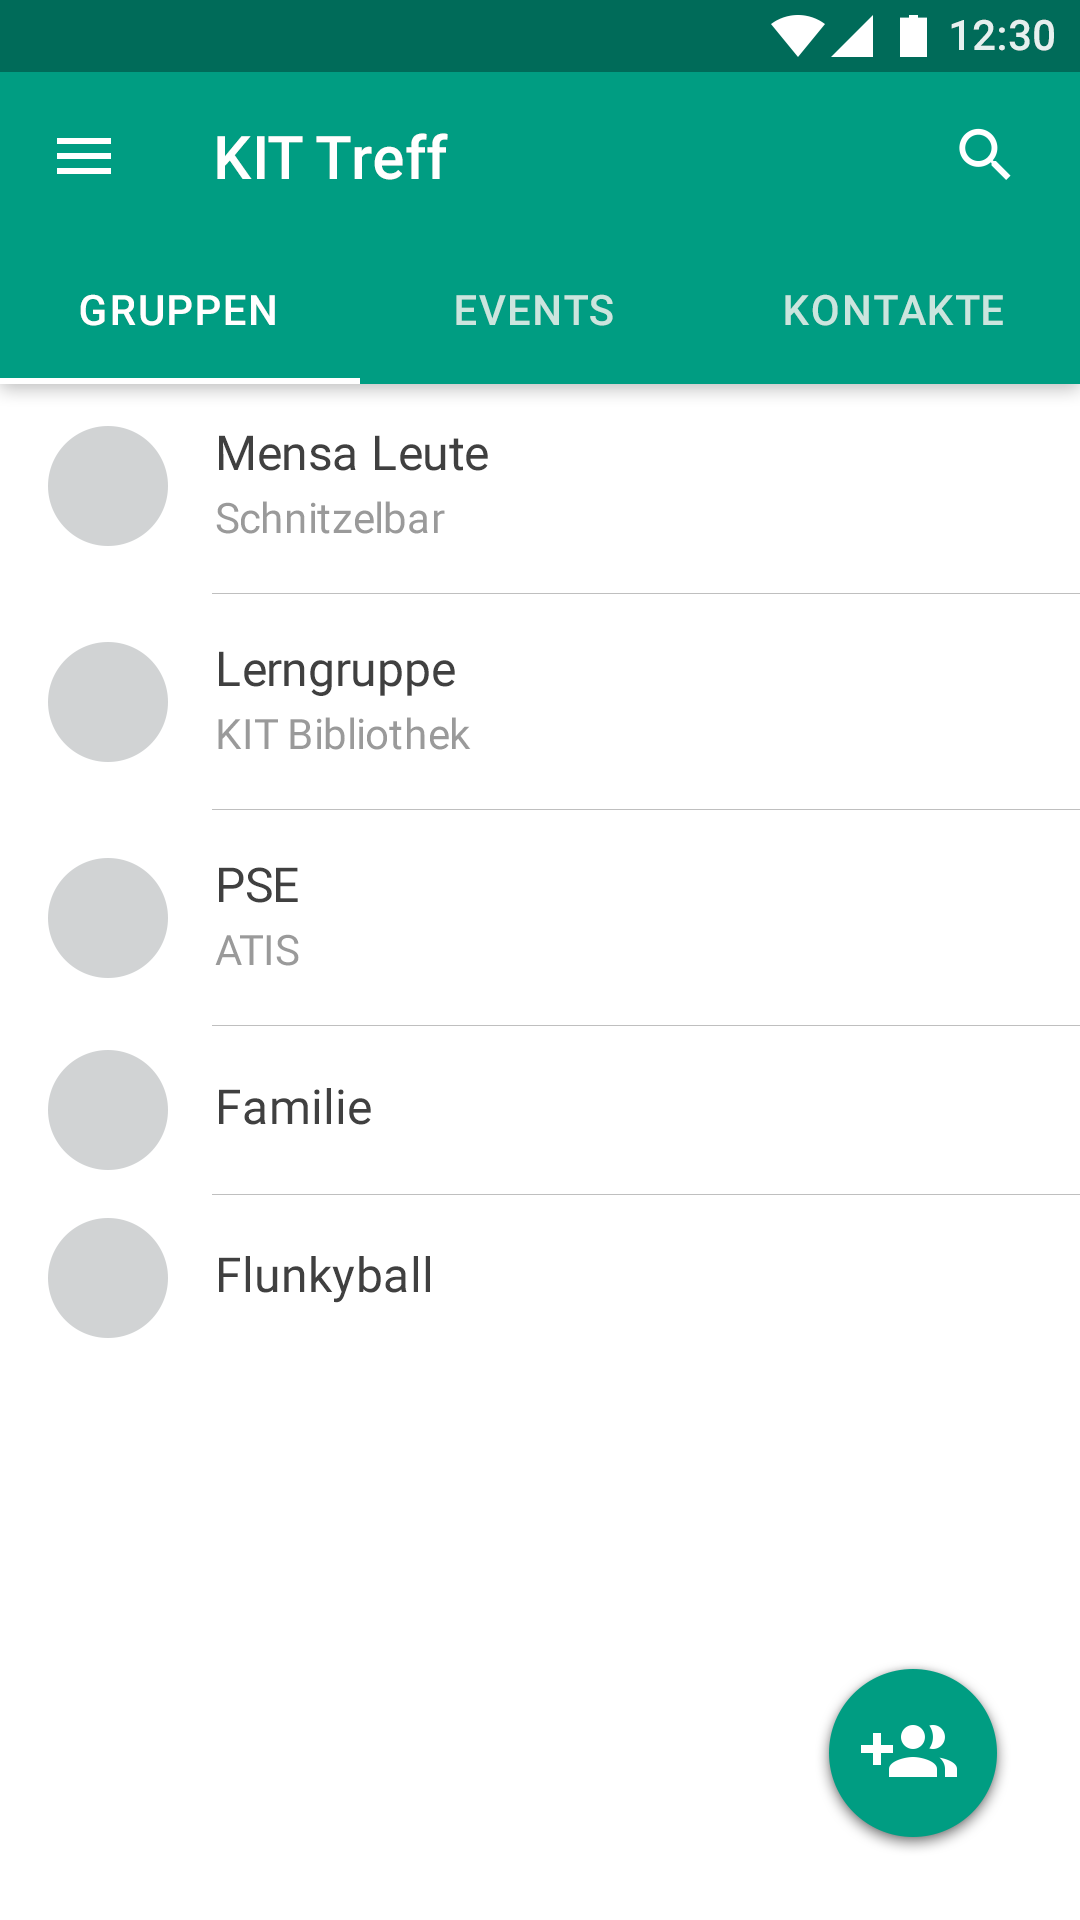
\includegraphics[height=80mm]{mockups/home_groups.png}}
	\caption{\label{fig:groups}
		Hier können Gruppen verwaltet und angesehen, sowie neue hinzugefügt werden.
		\testlink{tst:grpcreate}.
	}
\end{figure}

\begin{figure}[hb]
		\fbox{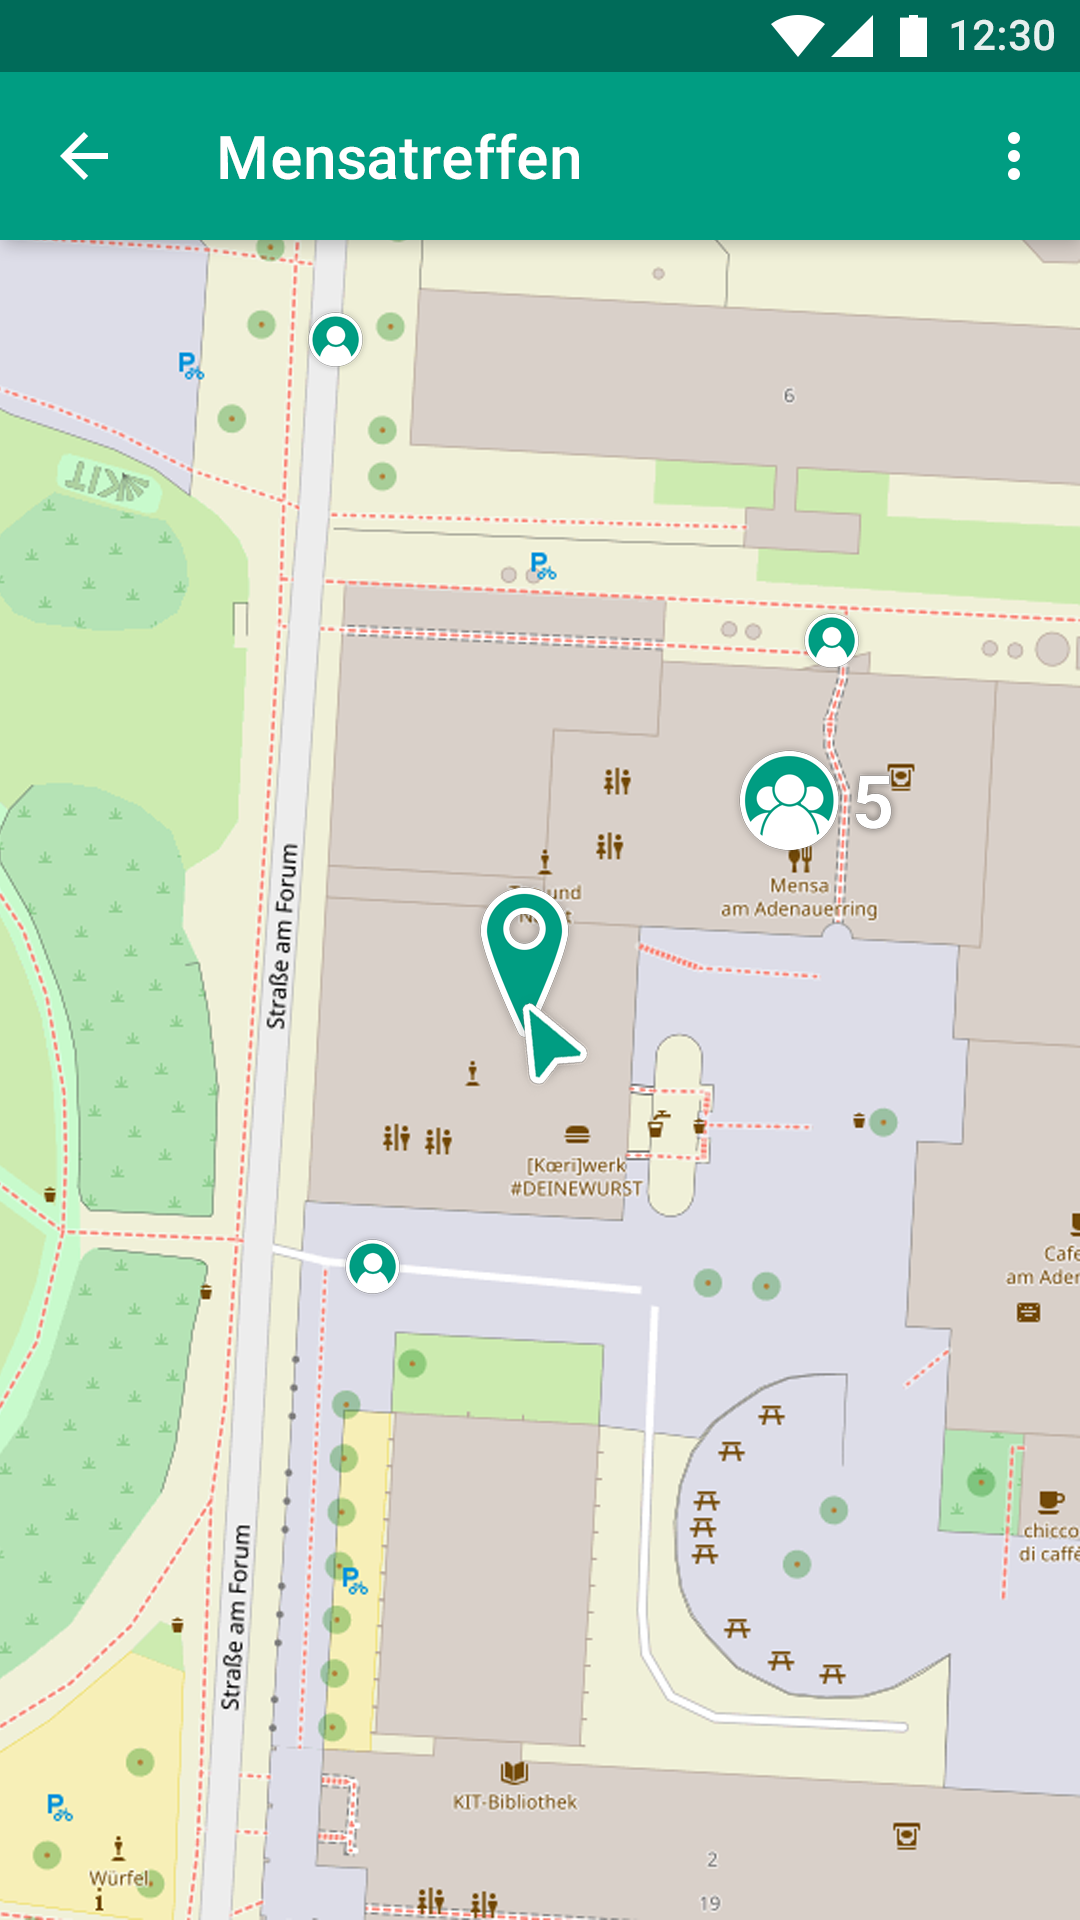
\includegraphics[height=80mm]{mockups/event_map.png}}
		\caption{\label{fig:map}
			Auf der Karte kann die Position der anderen Gruppenmitglieder eingesehen werden.
			Orte mit mehreren Mitgliedern erscheinen größer.
			\testlink{tst:grpcreate}.
		}
\end{figure}

\section{Glossar}

\textbf{Besucher}:
Eine Person, welche den Dienst nutzt.
Kann eingeloggt sein oder nicht.

\textbf{Nutzer}:
Ein eingeloggter Besucher.

\textbf{Gruppe}:
Mehrere Nutzer, welche untereinander Positionsdaten austauschen können.

\textbf{Chat}:
Möglichkeit für Mitglieder einer Gruppe, Textnachrichten auszutauschen.

\end{document}
